% This is text associated with the open textbook "Open Electromagnetics"
% See immediately below for author, date
% This work is licensed under the Creative Commons Attribution-ShareAlike 4.0 International License. (CC BY-SA 4.0) 
% To view a copy of the license, visit http://creativecommons.org/licenses/by-sa/4.0/

%ORB TITLE Plane Waves at Normal Incidence on a Material Slab
%ORB AUTHOR 0        # S.W. Ellingson, Virginia Tech (ellingson@vt.edu)
%ORB DATE 20191116   # yyyymmdd
%ORB ABSTRACT 

\label{m0162_Waves_at_Double_Planar_Boundary} % <-- Must match name of this file and module directory name.  Don't mess with this!
\index{slab|(}

In Section~\ref{m0161_Waves_at_Planar_Boundary}, we considered what happens when a uniform plane wave is normally incident on the planar boundary between two semi-infinite media.
In this section, we consider the problem shown in Figure~\ref{m0162_fPlaneWaveNormalIncidenceSlab}:
a uniform plane wave normally incident on a ``slab'' 
sandwiched between two semi-infinite media.  This scenario arises in many practical engineering problems, including the design and analysis of filters and impedance-matching devices at RF and optical frequencies, the analysis of RF propagation through walls, and the design and analysis of radomes.  
\index{radome}
The findings of Section~\ref{m0161_Waves_at_Planar_Boundary} are an important stepping stone to the solution of this problem, so a review of Section~\ref{m0161_Waves_at_Planar_Boundary} is recommended before reading this section.
\index{radome}
%
\begin{figure}[b!]
\begin{center}
\pdftooltip{{  % note double braces
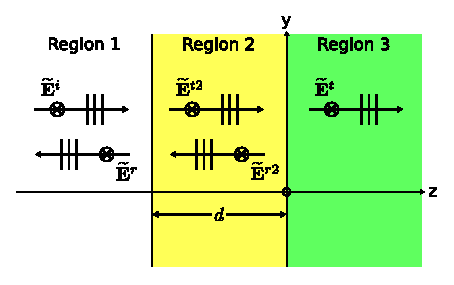
\includegraphics[width=0.8\columnwidth]{modules/m0162_fPlaneWaveNormalIncidenceSlab.eps} 
% https://commons.wikimedia.org/wiki/File:Upw_incident_on_a_slab.svg
}}{For a z-y coordinate system, plane wave normally incident on a slab. The positive z region is Region 3. Region 2 extends in the negative z direction a distance d. The remaining negative z area is Region 1. Regions 1 and 2 have real and imaginary parts of capital e tilde. Region 3 has capital e tilde superscript t.}
\end{center}
\centerline{\scriptsize 
\copyright~\hyperref[m0162_fPlaneWaveNormalIncidenceSlab_Credit]{C.\ Wang} 
\href{https://creativecommons.org/licenses/by-sa/4.0/}{CC BY-SA 4.0} 
} 
\caption{
\label{m0162_fPlaneWaveNormalIncidenceSlab}
A uniform plane wave normally incident on a slab.
}
\end{figure}

For consistency of terminology, let us refer to the problem considered in Section~\ref{m0161_Waves_at_Planar_Boundary} as the ``single-boundary'' problem and the present (slab) problem as the ``double-boundary'' problem.
Whereas there are only two regions (``Region 1'' and ``Region 2'') in the single-boundary problem, in the double-boundary problem there is a third region that we shall refer to as ``Region~3.''
We assume that the media comprising each slab are ``simple'' and lossless (i.e., the imaginary component of permittivity $\epsilon''$ is equal to zero) and therefore the media are completely defined by a real-valued permittivity and a real-valued permeability.
The boundary between Regions~1 and 2 is at $z=-d$, and the boundary between Regions~2 and 3 is at $z=0$.
Thus, the thickness of the slab is $d$.
In both problems, we presume an incident wave in Region~1 incident on the boundary with Region~2 having electric field intensity
%
\begin{equation}
\widetilde{\bf E}^i(z) = \hat{\bf x} E_0^i e^{-j\beta_1 z}~~~\mbox{(Region~1)}
\label{m0162_eEi}
\end{equation}
%
where $\beta_1=\omega\sqrt{\mu_1 \epsilon_1}$ is the phase propagation constant in Region~1. 
$\widetilde{\bf E}^i$ serves as the ``stimulus'' in this problem.
That is, all other contributions to the total field may be expressed in terms of $\widetilde{\bf E}^i$.

From the plane wave relationships, we determine that the associated magnetic field intensity is
%
\begin{equation}
\widetilde{\bf H}^i(z) = \hat{\bf y} \frac{E_0^i}{\eta_1}  e^{-j\beta_1 z}~~~\mbox{(Region~1)}
\label{m0162_eHi}
\end{equation}
%
where $\eta_1=\sqrt{\mu_1 / \epsilon_1}$ is the wave impedance in Region~1.

The symmetry arguments of the single-boundary problem apply in precisely the same way to the double-boundary problem.
Therefore, we presume that the reflected electric field intensity is:
%
\begin{equation}
\widetilde{\bf E}^r(z) = \hat{\bf x} B e^{+j\beta_1 z}~~~\mbox{(Region~1)}
\label{m0162_eEr}
\end{equation}
%
where $B$ is a complex-valued constant that remains to be determined;
and subsequently the reflected magnetic field intensity is:
%
\begin{equation}
\widetilde{\bf H}^r(z) = -\hat{\bf y} \frac{B}{\eta_1} e^{+j\beta_1 z}~~~\mbox{(Region~1)}
\label{m0162_eHr}
\end{equation}

Similarly, we infer the existence of a transmitted plane wave propagating in the $+\hat{\bf z}$ direction in Region~2.
The electric and magnetic field intensities of this wave are given by:
%
\begin{equation}
\widetilde{\bf E}^{t2}(z) = \hat{\bf x} C e^{-j\beta_2 z}~~~\mbox{(Region~2)}
\label{m0162_eEt}
\end{equation}
%
and an associated magnetic field having the form:
%
\begin{equation}
\widetilde{\bf H}^{t2}(z) = \hat{\bf y} \frac{C}{\eta_2} e^{-j\beta_2 z}~~~\mbox{(Region~2)}
\label{m0162_eHt}
\end{equation}
%
where $\beta_2=\omega\sqrt{\mu_2 \epsilon_2}$ and $\eta_2=\sqrt{\mu_2 / \epsilon_2}$ are the phase propagation constant and wave impedance, respectively, in Region~2.
The constant $C$, like $B$, is a complex-valued constant that remains to be determined.

Now let us consider the boundary between Regions~2 and 3.
Note that $\widetilde{\bf E}^{t2}$ is incident on this boundary in precisely the same manner as $\widetilde{\bf E}^i$ is incident on the boundary between Regions~1 and 2.
Therefore, we infer a reflected electric field intensity in Region~2 as follows: 
%
\begin{equation}
\widetilde{\bf E}^{r2}(z) = \hat{\bf x} D e^{+j\beta_2 z}~~~\mbox{(Region~2)}
\label{m0162_eEr2}
\end{equation}
%
where $D$ is a complex-valued constant that remains to be determined;
and an associated magnetic field
%
\begin{equation}
\widetilde{\bf H}^{r2}(z) = -\hat{\bf y} \frac{D}{\eta_2} e^{+j\beta_2 z}~~~\mbox{(Region~2)}
\label{m0162_eHr2}
\end{equation}
%
Subsequently, we infer a transmitted electric field intensity in Region~3 as follows: 
%
\begin{equation}
\widetilde{\bf E}^{t}(z) = \hat{\bf x} F e^{-j\beta_3 z}~~~\mbox{(Region~3)}
\label{m0162_eEt3}
\end{equation}
%
and an associated magnetic field having the form
%
\begin{equation}
\widetilde{\bf H}^{t}(z) = \hat{\bf y} \frac{F}{\eta_3} e^{-j\beta_3 z}~~~\mbox{(Region~3)}
\label{m0162_eHt3}
\end{equation}
%
where $\beta_3=\omega\sqrt{\mu_3 \epsilon_3}$ and $\eta_3=\sqrt{\mu_3 / \epsilon_3}$ are the phase propagation constant and wave impedance, respectively, in Region~3.
The constant $F$, like $D$, is a complex-valued constant that remains to be determined.
We infer no wave traveling in the ($-\hat{\bf z}$) in Region~3, just as we inferred no such wave in Region~2 of the single-boundary problem.

For convenience, Table~\ref{m0162_tFieldComponents} shows a complete summary of the field components we have just identified. 
%
\begin{table*}[t] % <-- forces table to span both columns (i.e., entire page width) at the top of the page
\begin{center}
\begin{tabular}{llll}
         & Electric Field Intensity & Magnetic Field Intensity & Region of Validity \\
\hline\hline
Region~1 & $\widetilde{\bf E}^i(z)    = \hat{\bf x} E_0^i e^{-j\beta_1 z}$    &  $\widetilde{\bf H}^i(z)    = +\hat{\bf y} \left(E_0^i/\eta_1\right) e^{-j\beta_1 z}$   &  $z \le -d$ \\
~        & $\widetilde{\bf E}^r(z)    = \hat{\bf x} B e^{+j\beta_1 z}$  &  $\widetilde{\bf H}^r(z)    = -\hat{\bf y} \left(B/\eta_1\right) e^{+j\beta_1 z}$ &  ~ \\
\hline
Region~2 & $\widetilde{\bf E}^{t2}(z) = \hat{\bf x} C e^{-j\beta_2 z}$  &  $\widetilde{\bf H}^{t2}(z) = +\hat{\bf y} \left(C/\eta_2\right) e^{-j\beta_2 z}$ &  $-d \le z \le 0$ \\
~        & $\widetilde{\bf E}^{r2}(z) = \hat{\bf x} D e^{+j\beta_2 z}$  &  $\widetilde{\bf H}^{r2}(z) = -\hat{\bf y} \left(D/\eta_2\right) e^{+j\beta_2 z}$ &  ~ \\
\hline
Region~3 & $\widetilde{\bf E}^t(z)    = \hat{\bf x} F e^{-j\beta_3 z}$  &  $\widetilde{\bf H}^t(z)    = +\hat{\bf y} \left(F/\eta_3\right) e^{-j\beta_3 z}$ &  $z \ge 0$
\end{tabular}
\end{center}
\caption{\label{m0162_tFieldComponents} Field components in the double-boundary (slab) problem of Figure~\ref{m0162_fPlaneWaveNormalIncidenceSlab}.}
\end{table*}
%
Note that the \emph{total} field intensity in each region is the \emph{sum} of the field components in that region.
For example, the total electric field intensity in Region~2 is $\widetilde{\bf E}^{t2}+\widetilde{\bf E}^{r2}$.

Now observe that there are four unknown constants remaining; namely $B$, $C$, $D$, and $F$.  
The double-boundary problem is completely solved once we have expressions for these constants in terms of the ``given'' quantities in the problem statement.
Solutions for the unknown constants can be obtained by enforcing boundary conditions on the electric and magnetic fields at each of the two boundaries.
As in the single-boundary case, the relevant boundary condition is that the total field should be continuous across each boundary.
Applying this condition to the boundary at $z=0$, we obtain:
%
\begin{equation}
\widetilde{\bf E}^{t2}(0) + \widetilde{\bf E}^{r2}(0) = \widetilde{\bf E}^{t}(0) 
\label{m0162_eB1E}
\end{equation}
%
\begin{equation}
\widetilde{\bf H}^{t2}(0) + \widetilde{\bf H}^{r2}(0) = \widetilde{\bf H}^{t}(0)
\label{m0162_eB1H}
\end{equation}
%
Applying this condition to the boundary at $z=-d$, we obtain:
%
\begin{equation}
\widetilde{\bf E}^i(-d) + \widetilde{\bf E}^r(-d)  = \widetilde{\bf E}^{t2}(-d) + \widetilde{\bf E}^{r2}(-d)
\label{m0162_eB2E}
\end{equation}
%
\begin{equation}
\widetilde{\bf H}^i(-d) + \widetilde{\bf H}^r(-d)  = \widetilde{\bf E}^{t2}(-d) + \widetilde{\bf E}^{r2}(-d)
\label{m0162_eB2H}
\end{equation}
%
Making substitutions from Table~\ref{m0162_tFieldComponents} and dividing out common factors, Equation~\ref{m0162_eB1E} becomes:
%
\begin{equation}
C + D =F
\label{m0162_eB1Es}
\end{equation}
%
Equation~\ref{m0162_eB1H} becomes:
%
\begin{equation}
\frac{C}{\eta_2} - \frac{D}{\eta_2}  = \frac{F}{\eta_3} 
\label{m0162_eB1Hs}
\end{equation}
%
Equation~\ref{m0162_eB2E} becomes:
%
\begin{equation}
E_0^i e^{+j\beta_1 d} + B e^{-j\beta_1 d}  = C e^{+j\beta_2 d} + D e^{-j\beta_2 d}
\label{m0162_eB2Es}
\end{equation}
Equation~\ref{m0162_eB2H} becomes:
%
\begin{equation}
\frac{E_0^i}{\eta_1} e^{+j\beta_1 d} - \frac{B}{\eta_1} e^{-j\beta_1 d} = \frac{C}{\eta_2} e^{+j\beta_2 d} - \frac{D}{\eta_2} e^{-j\beta_2 d}
\label{m0162_eB2Hs}
\end{equation}

Equations~\ref{m0162_eB1Es}--\ref{m0162_eB2Hs} are recognizable as a system of 4 simultaneous linear equations with the number of unknowns equal to the number of equations.  
We could simply leave it at that, however, some very useful insights are gained by solving this system of equations in a particular manner.
First, note the resemblance between the situation at the $z=0$ boundary in this problem and the situation at $z=0$ boundary in the single-boundary problem.  
In fact, the two are the {\it same} problem, with the following transformation of variables (single-boundary $\rightarrow$ double-boundary):
%
\begin{equation}
E_0^i \rightarrow C ~~~\mbox{i.e., the independent variable}
\end{equation}  
%
\begin{equation}
B \rightarrow D ~~~\mbox{i.e., reflection}
\end{equation} 
%
\begin{equation}
C \rightarrow F ~~~\mbox{i.e., transmission}
\end{equation} 
%
It immediately follows that 
%
\begin{equation}
D = \Gamma_{23} C 
\end{equation}
%
and
%
\begin{equation}
F = \left(1+\Gamma_{23}\right) C   
\end{equation}
%
where
%
\begin{equation}
\boxed{
\Gamma_{23}  \triangleq \frac{\eta_3-\eta_2}{\eta_3+\eta_2} 
}
\label{m0162_eGamma23}
\end{equation} 

At this point, we could use the expressions we have just derived to eliminate $D$ and $F$ in the system of four simultaneous equations identified earlier.
This would reduce the problem to that of two equations in two unknowns -- a dramatic simplification!  

However, even this is more work than is necessary, and a little cleverness at this point pays big dividends later.  The key idea is that we usually have no interest in the fields internal to the slab; in most problems, we are interested merely in reflection into Region~1 from the $z=-d$ boundary and transmission into Region~3 through the $z=0$ interface.  
With this in mind, let us simply replace the two-interface problem in Figure~\ref{m0162_fPlaneWaveNormalIncidenceSlab} with an ``equivalent'' single-boundary problem shown in Figure~\ref{m0162_fPlaneWaveNormalIncidenceSlabEq}.  This problem is ``equivalent'' in the following sense only:
Fields in Region~1 are identical to those in Region~1 of the original problem.  
The material properties in the region to the right of the $z=-d$ boundary in the equivalent problem seem unlikely to be equal to those in Regions~2 or 3 of the original problem, so we define a new wave impedance $\eta_{eq}$ to represent this new condition.  If we can find an expression for $\eta_{eq}$, then we can develop a solution to the original (two-boundary) problem that looks like a solution to the equivalent (simpler, single-boundary) problem.
%
\begin{figure}
\begin{center}
\pdftooltip{{  % note double braces
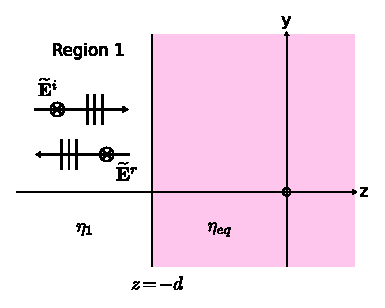
\includegraphics[width=0.8\columnwidth]{modules/m0162_fPlaneWaveNormalIncidenceSlabEq.eps} 
% https://commons.wikimedia.org/wiki/File:Double-boundary_problem_equivalent.svg
}}{For a z-y coordinate system, region 1 defined as in Figure 5.2. Regions 2 and 3 are combined into a single region. Region 1 labeled small eta subscript 1. Combined region labeled small eta subscript eq.}
\end{center}
\centerline{\scriptsize 
\copyright~\hyperref[m0162_fPlaneWaveNormalIncidenceSlabEq_Credit]{C.\ Wang} 
\href{https://creativecommons.org/licenses/by-sa/4.0/}{CC BY-SA 4.0} 
} 
\caption{
\label{m0162_fPlaneWaveNormalIncidenceSlabEq}
Representing the double-boundary problem as an equivalent single-boundary problem.
}
\end{figure}

To obtain an expression for $\eta_{eq}$, we invoke the definition of wave impedance:  It is simply the ratio of electric field intensity to magnetic field intensity in the medium.  Thus:
%
\begin{equation}
\eta_{eq}  
\triangleq \frac{ \hat{\bf x} \cdot \widetilde{\bf E}_2(z_2) }{ \hat{\bf y} \cdot \widetilde{\bf H}_2(z_2) }
= \frac{ \hat{\bf x} \cdot \left[ \widetilde{\bf E}^{t2}(z_2) + \widetilde{\bf E}^{r2}(z_2) \right] }{ \hat{\bf y} \cdot  \left[ \widetilde{\bf H}^{t2}(z_2) + \widetilde{\bf H}^{r2}(z_2) \right]  }
\end{equation}
%
where $z_2$ is any point in Region~2.  For simplicity, let us choose $z_2 = -d$.  Making substitutions, we obtain:  
%
\begin{equation}
\eta_{eq}  
= \frac{ C e^{+j\beta_2 d} + D e^{-j\beta_2 d} }{ \left(C/\eta_2\right) e^{+j\beta_2 d} - \left(D/\eta_2\right) e^{-j\beta_2 d} }
\end{equation}
%
Bringing the factor of $\eta_2$ to the front and substituting $D = \Gamma_{23} C$:
%
\begin{equation}
\eta_{eq}  
= \eta_2 \frac{ C e^{+j\beta_2 d} + \Gamma_{23} C e^{-j\beta_2 d} }{ C e^{+j\beta_2 d} - \Gamma_{23} C e^{-j\beta_2 d} }
\end{equation}
%
Finally, we divide out the common factor of $C$ and multiply numerator and denominator by $e^{-j\beta_2 d}$, yielding:
%
\begin{equation}
\boxed{
\eta_{eq}  
= \eta_2 \frac{ 1 + \Gamma_{23} e^{-j2\beta_2 d} }{ 1 - \Gamma_{23} e^{-j2\beta_2 d} }
}
\label{m0162_eetaeq}
\end{equation}
%
%%%%%%%%%%%%%%%%%%%%%%%%%%%%%%%%%%%%%%%%%%%%%%%
%ORB HIGHLIGHT
\begin{mdframed}[backgroundcolor=yellow!20,nobreak=true] 
Equation~\ref{m0162_eetaeq} is the wave impedance in the region to the right of the boundary in the equivalent scenario shown in Figure~\ref{m0162_fPlaneWaveNormalIncidenceSlabEq}.  ``Equivalent'' in this case means that the incident and reflected fields in Region~1 are identical to those in the original (slab) problem. 
\end{mdframed}
%%%%%%%%%%%%%%%%%%%%%%%%%%%%%%%%%%%%%%%%%%%%%%%

Two comments on this expression before proceeding.  
First: Note that if the materials in Regions~2 and 3 are identical, then $\eta_2=\eta_3$, so $\Gamma_{23}=0$, and thus $\eta_{eq}=\eta_2$, as expected.  
Second: Note that $\eta_{eq}$ is, in general, complex-valued.  
This may initially seem troubling, since the imaginary component of the wave impedance is normally associated with general (e.g., possibly lossy) material.
We specifically precluded this possibility in the problem statement, so clearly the complex value of the wave impedance is not indicating loss.
Instead, the non-zero phase of $\eta_{eq}$ represents the ability of the standing wave 
\index{standing wave}
inside the slab to impart a phase shift between the electric and magnetic fields.
This is \emph{precisely} the same effect that one observes at the input of a transmission line: 
\index{transmission line!analogy for wave propagation}
The input impedance $Z_{in}$ is, in general, complex-valued even if the line is lossless and the characteristic impedance and load impedance are real-valued.\footnote{See the section ``Input Impedance of a Terminated Lossless Transmission Line'' for a reminder.  This section may appear in a different volume depending on the version of this book.}
In fact, the impedance looking into a transmission line is given by an expression of precisely the same form as Equation~\ref{m0162_eetaeq}.
This striking analogy between plane waves at planar boundaries and voltage and current waves in transmission lines applies broadly. 

We can now identify an ``equivalent reflection coefficient'' $\Gamma_{1,eq}$ for the scenario shown in Figure~\ref{m0162_fPlaneWaveNormalIncidenceSlabEq}:
%
\begin{equation}
\boxed{
\Gamma_{1,eq}  \triangleq \frac{\eta_{eq}-\eta_1}{\eta_{eq}+\eta_1} 
}
\end{equation} 
%
The quantity $\Gamma_{1,eq}$ may now be used precisely in the same way as $\Gamma_{12}$ was used in the single-boundary problem to find the reflected fields and reflected power density in Region~1.

%%%%%%%%%%%%%%%%%%%%%%%%%%%%%%%%%%%%%%%%%%%%%%%
%ORB EXAMPLE
~\\ \begin{example} 
\label{m0162_exWiFi}
\begin{mdframed}[backgroundcolor=brown!20,linecolor=brown!20]\raggedright
Reflection of WiFi from a glass pane.
\\~\\
A WiFi (wireless LAN) signal at a center frequency of 2.45~GHz is normally incident on a glass pane which is 1~cm thick and is well-characterized in this application as a lossless dielectric with $\epsilon_r=4$.
The source of the signal is sufficiently distant from the window that the incident signal is well-approximated as a plane wave.
Determine the fraction of power reflected from the pane.\\
~\\

\noindent
{\bf Solution.} In this case, we identify Regions~1 and 3 as approximately free space, and Region~2 as the pane.
Thus 
%
\begin{equation}
\eta_1=\eta_3=\eta_0 \cong 376.7~\Omega
\end{equation}
%
and
%
\begin{equation}
\eta_2=\frac{\eta_0}{\sqrt{\epsilon_r}} \cong 188.4~\Omega
\end{equation}
%
The reflection coefficient from Region~2 to Region~3 is
%
\begin{flalign}
\Gamma_{23} &= \frac{\eta_3-\eta_2}{\eta_3+\eta_2} \nonumber \\
            &= \frac{\eta_0-\eta_2}{\eta_0+\eta_2} \nonumber \\
            &\cong 0.3333 
\end{flalign}
%
Given $f=2.45$~GHz, the phase propagation constant in the glass is
%
\begin{equation}
\beta_2 = \frac{2\pi}{\lambda} = \frac{2\pi f\sqrt{\epsilon_r}}{c} \cong 102.6~\mbox{rad/m} 
\end{equation}
%
Given $d=1$~cm, the equivalent wave impedance is
%
\begin{flalign}
\eta_{eq}  &= \eta_2 \frac{ 1 + \Gamma_{23} e^{-j2\beta_2 d} }{ 1 - \Gamma_{23} e^{-j2\beta_2 d} } \nonumber \\
           &\cong 117.9 -j78.4~\Omega
\end{flalign}
%
Next we calculate
%
\begin{flalign}
\Gamma_{1,eq} &= \frac{\eta_{eq}-\eta_1}{\eta_{eq}+\eta_1} \nonumber \\
              &\cong -0.4859 -j0.2354 
\end{flalign}
%
The ratio of reflected power density to incident power density is simply the squared magnitude of this reflection coefficient, i.e.:
%
\begin{equation}
\frac{S_{ave}^r}{S_{ave}^i} = \left|\Gamma_{1,eq}\right|^2 = 0.292 \cong \boxed{\mbox{29.2\%}} 
\end{equation}
%
where $S_{ave}^r$ and $S_{ave}^i$ are the reflected and incident power densities, respectively. 
\end{mdframed}
% note figures will need to go between "\end{mdframed}" and "\end{example}"
\end{example}
%%%%%%%%%%%%%%%%%%%%%%%%%%%%%%%%%%%%%%%%%%%%%%%

Since $B=\Gamma_{1,eq}E_0^i$, we have:
%
\begin{equation}
\widetilde{\bf E}^r(z) = \hat{\bf x} \Gamma_{1,eq} E_0^i e^{+j\beta_1 z}~\mbox{,}~~z \le -d
\end{equation}
%
and $\widetilde{\bf H}^r(z)$ can be obtained from the plane wave relationships. 
If desired, it is now quite simple to obtain solutions for the electric and magnetic fields in Regions~2 and 3.
However, it is the usually the power density transmitted into Region~3 that is of greatest interest.
This power density is easily determined from the principle of conservation of power.
If the loss in Region~2 is negligible, then no power can be dissipated there.
In this case, all power not reflected from the $z=-d$ interface must be transmitted into Region~3.
In other words:
%
\begin{equation}
\boxed{ \frac{S_{ave}^t}{S_{ave}^i} = 1-|\Gamma_{1,eq}|^2 } 
\label{m0162_eSavet}
\end{equation} 
%
where $S_{ave}^t$ is the transmitted power density. 

%%%%%%%%%%%%%%%%%%%%%%%%%%%%%%%%%%%%%%%%%%%%%%%
%ORB EXAMPLE
~\\ \begin{example} 
\begin{mdframed}[backgroundcolor=brown!20,linecolor=brown!20]\raggedright
Transmission of WiFi through a glass pane.
\\~\\
Continuing Example~\ref{m0162_exWiFi}: What fraction of incident power passes completely through the glass pane?\\
~\\

\noindent
{\bf Solution.} 
%
\begin{equation}
\frac{S_{ave}^t}{S_{ave}^i} = 1-|\Gamma_{1,eq}|^2 \cong \boxed{\mbox{70.8\%}}
\end{equation}
%
\end{mdframed}
% note figures will need to go between "\end{mdframed}" and "\end{example}"
\end{example}

%%%%%%%%%%%%%%%%%%%%%%%%%%%%%%%%%%%%%%%%%%%%%%%
{\bf Additional Reading:}
\begin{itemize}
\item ``\href{https://en.wikipedia.org/wiki/Radome}{Radome}'' on Wikipedia.
\end{itemize}

\index{slab|)}
